\documentclass[11pt, a4paper]{article}
\usepackage[left=12mm, right=12mm, top=20mm, bottom=20mm]{geometry}


\usepackage{fancyhdr}
\usepackage{graphicx}

\pagestyle{fancy}


% Header
\lhead{
\includegraphics[width=5cm]{fhnwlogo.pdf}}
\chead{}
\rhead{DIST - BloomFilter}
\renewcommand{\headrulewidth}{0.4pt}
%Footer
\lfoot{Autoren: Damian Zehnder, Mario Wettstein}
\cfoot{}
\rfoot{\thepage} 
\renewcommand{\footrulewidth}{0.1pt}

% Alphabetic Sections%
\renewcommand*{\thesection}{\Alph{section}}


\begin{document}

\section*{BloomFilter}


\section{Idee des Bloom-Filters}
Ein BloomFilter liefert schnell eine Antwort, ob ein Wert bereits vorgekommen ist oder nicht. \\\\
Der Filter liefert also zwei verschiedene Antworten:
\begin{itemize}  
	\item Mit hoher Wahrscheinlichkeit enthalten
	\item Definitiv nicht enthalten
\end{itemize}
Gerade das ein Wert nicht bekannt ist, kann genutzt werden, um schnelle Entscheidungen zu treffen.\\





\begin{tabular}{ |p{8cm}||p{8cm}|  }
	\hline
	\multicolumn{2}{|c|}{Vor- und Nachteile} \\
	\hline
	Vorteil&Nachteil\\
	\hline
	\begin{itemize}  
		\item sehr performant
		\item Treffergenauigkeit {\H u}ber die Gr{\H o}sse des Index konfigurierbar, dabei besteht kein Risiko, dass ein Treffer nicht gefunden wird 
		\item kompaktes Speichern der Daten (oft wird nur circa 1/8 der Ausgangs-Datenmenge ben{\H o}tigt) 
		\item Implementierungen in allen relevanten Programmiersprachen verf{\H u}gbar 
		\item leicht parallelisierbar ({\H u}ber Aufteilung des Suchindex auf mehrere Server/CPU-Kerne) 
	\end{itemize}
	&
	\begin{itemize}  
		\item keinerlei {\H A}hnlichkeitssuche, keine Fehlertoleranz 
		\item Suchergebnisse werden nicht sortiert 
		\item Risiko, sogenannte False Positives zu erhalten, das heisst, es k{\H o}nnen Datens{\H a}tze zur{\H u}ckgegeben werden, die den Suchbegriff nicht enthalten 
	\end{itemize}
	\\
	\hline
\end{tabular}





\section{Praxisbeispiel}

\includegraphics[height=8mm]{image/Ethereum.png}
Ethereum benutzt einen Bloom Filter,\\ um Logs schnell und effizient in der Ethereum Blockchain finden zu k{\H o}nnen. \\
\\
Im Ethereum-System m{\H u}ssen Events, einschließlich historischer Events, leicht und ohne unn{\H o}tigen Aufwand gefiltert und gesucht werden k{\H o}nnen. Gleichzeitig ist der Speicherplatz teuer, dass nicht viele Daten gespeichert werden sollen, wie z. B. die Liste der Transaktionen und die von ihnen erstellten Protokolle.
Wenn ein Block generiert oder veifiziert wird, wird die Adresse eines Protokollierungsvertrags einem Bloom Filter hinzugef{\H u}gt, der im Blockheader enthalten ist. Die eigentlichen Protokolle sind aus Platzgr{\H u}nden nicht in den Blockdaten enthalten.
Wenn nun alle Protokolleintr{\H a}ge durchsucht werden, kann der Bloom Filter {\H u}berpr{\H u}fen, ob relevante Protokolle vorhanden sind.

\section{Testen der Fehlerwahrscheinlichkeit}

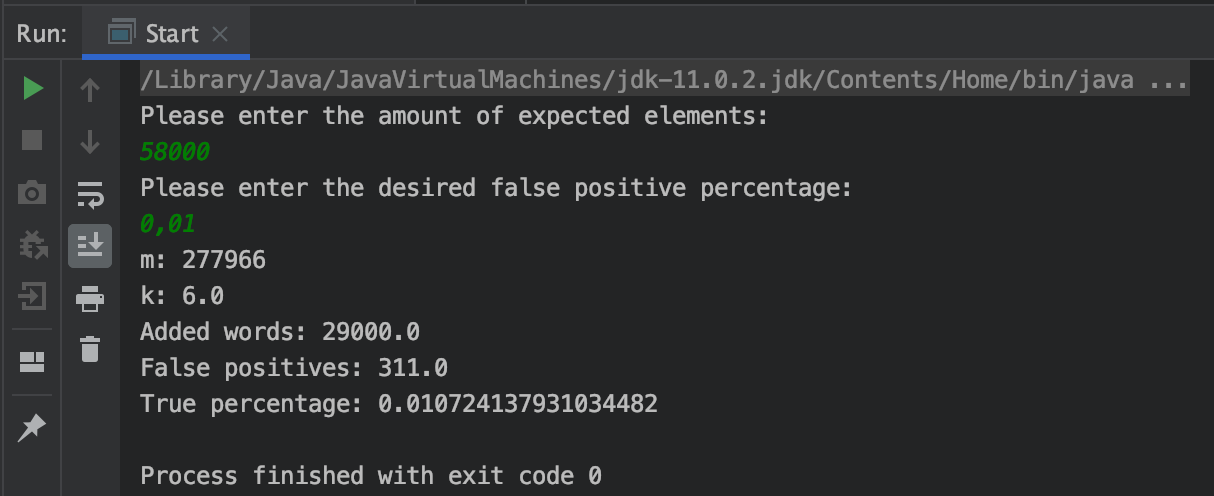
\includegraphics[width=10cm]{image/Result.png}\\
Die Fehlerwahrscheinlichkeit wird in unserem Programm folgendermassen berechnet:
Zuerst kann der Benutzer eine bestimmte anzahl W{\H o}rter angeben, die in seinem Datensatz vorhanden sind und eine gew{\H u}nschte Fehlertoleranz in Prozent.\\
\\
Der Bloom Filter berechnet aus diesen beiden Werten die geeignete Bit Array Gr{\H o}sse und die Anzahl Hash Funktionen.\\
\\
Das Programm f{\H u}gt jedes zweite Wort in die Bloom Filter Liste. Beim hinzuf{\H u}gen wird ein Hash Wert generiert, mithilfe der Google Guava Library.\\
Aus diesem Hash Wert wird ausgelesen, an welcher Position im Bit Array eine 1 gesetzt werden soll.\\
\\
Nachdem jedes zweite Wort hinzugef{\H u}gt wurde, wird die andere H{\H a}lfte der W{\H o}rter im Datensatz verglichen.\\
Dazu wird wieder aus jedem Wort ein Hash Wert generiert und es wird {\H u}berpr{\H u}ft, ob an der Stelle im Bit Array das Bit noch auf 0 gesetzt ist, was bedeutet dass das Wort nicht vorhanden ist.\\
\\
Aus der Anzahl hinzugef{\H u}gter W{\H o}rter und der Anzahl gefundenen W{\H o}rtern kann nun die eigentliche Prozentzahl berechnet werden.\\
\\
Diese liegt bei einem Datensatz von 58000 W{\H o}rtern bei einer Genauigkeit von {\H u}ber 99 \%.



\end{document}
